\documentclass[a4paper]{article}

\usepackage[margin=1in]{geometry}
\usepackage{amsmath}
\usepackage{amssymb}
\usepackage{graphicx}
\usepackage{float}
\usepackage{hyperref}
\usepackage[outputdir=out]{minted}
\usepackage{subcaption}
\usepackage{amsfonts}
\usepackage{pdfpages}
\usepackage[justification=centering]{caption}
\usepackage{algpseudocode}

\def\sectionautorefname{Section}
\def\subsectionautorefname{Section}
\def\subsubsectionautorefname{Section}
\def\figureautorefname{Figure}
\def\tableautorefname{Table}
\def\equationautorefname{Equation}


\begin{document}

    \title{Logistic Classification}
    \author{3F8 laboratory experiment \\ Theo A. Brown \\ Selwyn College, University of Cambridge}
    \date{\today}
    \maketitle

    \begin{abstract}
        Enter a short summary here.
    \end{abstract}

    \section{Introduction}\label{sec:introduction}
    Classification is the task of grouping data points according to their shared features, and assigning each group
    a label. This is often a trivial manual task for small datasets, but with very large collections of data it
    becomes very time intensive, so the development of good machine classifiers is an important area in statistical
    learning. Trained classifiers can be used as predictive tools to identify the most probable class that a new
    input will belong to, which could, for example, be useful in a medical setting, such as identifying the most
    at-risk patients.

    A key tool in classification is the ability to classify non-linear datasets, where the boundary between classes
    is not a straight line. This report explores the use of a set of non-linear basis functions (in this case,
    radial functions), which are applied to the inputs before classifying, to allow the discovery of non-linear
    decision boundaries.

    \section{Derivation of the gradient of the log-likelihood}\label{sec:gradient-derivation}
    If each datapoint's class label is assumed to be independent and identically generated from a Bernoulli distribution
    in which the probability of a class label is given by a logistic function applied to weighted inputs, the
    log-likelihood is as follows:
    \begin{align*}
        \mathcal{L}(w) = \log P(y|X, w) &= \log \prod_{n=1}^{N} \sigma(w^T \tilde{x}^{(n)})^{y^{(n)}}\sigma(-w^T \tilde{x}^{(n)})^{1-y^{(n)}} \\
        &= \sum_{n=1}^{N} y^{(n)} \log\sigma(w^T \tilde{x}^{(n)}) + (1-y^{(n)}) \log\sigma(-w^T \tilde{x}^{(n)})
    \end{align*}
    The derivative of the log-likelihood is calculated using the identities $\frac{d\sigma(x)}{dx} = \sigma(x)\sigma(-x)$
    and $\frac{d\log(x)}{dx} = \frac{1}{x}$. Applying the chain rule:
    \begin{align*}
        \frac{\partial \mathcal{L}}{\partial w} &= \sum_{n=1}^{N} y^{(n)} \sigma(-w^T \tilde{x}^{(n)}) \tilde{x}^{(n)} - (1-y^{(n)}) \sigma(w^T \tilde{x}^{(n)})  \tilde{x}^{(n)}
        \\ &= \sum_{n=1}^{N} \left(y^{(n)} - \sigma(w^T \tilde{x}^{(n)}) \right)  \tilde{x}^{(n)}
    \end{align*}

    \section{Gradient ascent algorithm}\label{sec:gradient-ascent-algorithm}
    To find the parameter $w$ that maximises the log-likelihood, the following gradient ascent algorithm is used:

    \begin{algorithmic}[1]
        \Procedure{GradientAscent}{X, y, n, r}
            \State $a \gets [1 \dots 1]^T$
            \State $\tilde{X} \gets [a ; X]$
            \State $w \gets [0 \dots 0]$
            \For{$i\gets 1, n$}
                \State $J \gets (y - (1 - \exp(\tilde{X} w))) \tilde{X}$
                \State $w \gets w + rJ$
            \EndFor
        \EndProcedure
    \end{algorithmic}

    In Python, this can be implemented as follows:

    \begin{minted}{python}
        import numpy as np

        def logistic(x):
            return 1 / (1 + np.exp(-x))

        def gradient_ascent(X, y,
                            number_iterations, learning_rate):
            # Prepend a column of ones to the input data (X)
            X1 = np.column_stack((np.ones(X.shape[0]), X))
            # Initialise the weights
            w = np.ones(X1.shape[1])

            for i in range(number_iterations):
                # Calculate the gradient
                dL = (y - logistic(X1 @ w)) @ X1
                # Move an amount proportional to the learning rate
                # in the direction of the gradient
                w += learning_rate * dL
            return w
    \end{minted}

    Note that the weights do not necessarily need to be initialised as ones - they could have been selected randomly, or
    initialised at zero, for example. The Python 3.5+ matrix multiplication operator $@$ is used to vectorise the
    operations.

    The \verb`learning_rate` parameter is chosen empirically. Starting with a value chosen such the algorithm shows signs
    of convergence, the learning rate is increased until the algorithm begins to oscillate. The rate is then decreased
    slightly so that the oscillation is avoided. Using this method, a fast rate of convergence is ensured and divergence
    avoided.

    \section{Data visualisation}\label{sec:data-visualisation}
    The data is visualised in the two-dimensional input space in \autoref{fig:data}. From the plot it is clear that a
    linear classifier will perform badly on the data, as the classes are not linearly separable: there is no straight
    boundary that successfully distinguishes between red and blue data points.

    \begin{figure}[h]
        \label{fig:data}
        \centering
        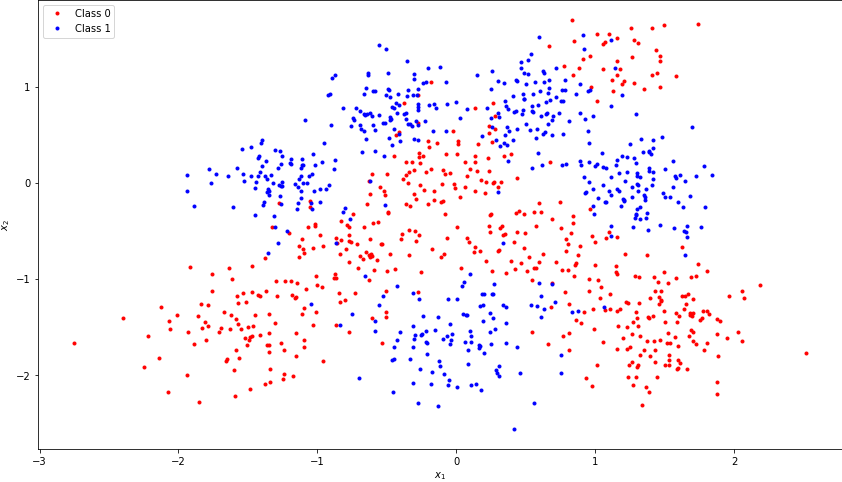
\includegraphics[width=0.8\textwidth]{plots/data.png}
        \caption{Plot of the two-dimensional input features (1000 datapoints, 2 classes)}
    \end{figure}

    \section{Model training}\label{sec:model-training}
    The data was split into a training set of 800 points and a test set of 200 points, and the gradient descent
    algorithm with a learning rate of 0.001 was applied to find the weights for the linear classifier. The mean
    log-likelihood (where the mean is taken across all of the weights) is plotted in \autoref{fig:log_likelihood} for
    the training and test datasets at each iteration.

    \begin{figure}[h]
        \label{fig:log_likelihood}
        \centering
        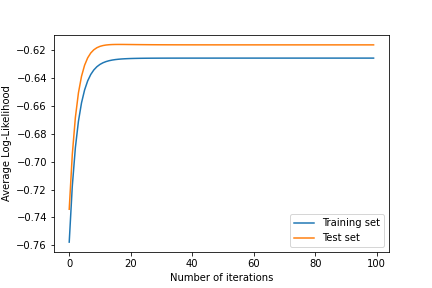
\includegraphics[width=0.8\textwidth]{plots/log_likelihood.png}
        \caption{Plot of the mean log-likelihood of the weights for the test and training data, over the
        course of model training}
    \end{figure}

    \autoref{fig:log_likelihood} shows that a plateau is reached for the log-likelihood of the parameters in both the
    training and test sets, after which no further improvements can be made. This suggests an optimum has been found for
    this model. After training there remains a difference between the performance on the test and training sets, which
    could suggest that the model with the given parameters has failed to capture the underlying pattern or has been
    overfitted. Additional metrics are required to assess the model performance further.

    \section{Model performance}\label{sec:model-performance}
    The predictive distribution of the model is shown in \autoref{fig:predictive_distribution_linear}. It is clear that
    this model fails to accurately classify the two classes. It identifies that the general principle that a greater
    proportion of the points with negative $x_2$ values are class 1 and more points with positive $x_2$ values are class
    2, but it is apparent to the human eye that this is overly simplified, failing to identify the islands of class 1 in
    class 2 and vice versa.

    \begin{figure}[h]
        \label{fig:predictive_distribution_linear}
        \centering
        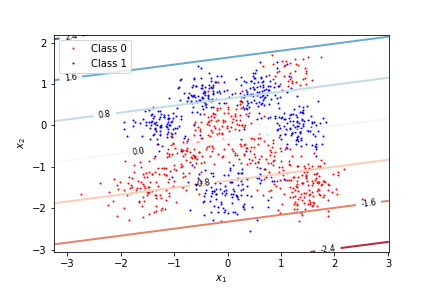
\includegraphics[width=0.8\textwidth]{plots/predictive_distribution_linear.png}
        \caption{Model predictive distribution overlaid on input datapoints, coloured by true classification}
    \end{figure}
\end{document}